\documentclass[11pt]{article}

\usepackage[utf8]{inputenc}
\usepackage[margin=1in]{geometry}
\usepackage{amsmath,amssymb}
\usepackage{mathptmx}
\usepackage{graphicx}
\usepackage{siunitx}
\usepackage{booktabs}
\usepackage{longtable}
\usepackage{xcolor}
\usepackage{caption}
\usepackage{float}
\usepackage{hyperref}
\hypersetup{colorlinks=true,linkcolor=blue,citecolor=blue,urlcolor=blue}
\renewcommand{\figurename}{Supplementary Fig.}
\renewcommand{\tablename}{Supplementary Table}
\setcounter{figure}{0}
\setcounter{table}{0}

\begin{document}

\begin{center}
{\Large \textbf{Supplementary Information}}\\[0.5em]
{\large Fungal Hyphae Reorganize Condensation Fields as Distributed Hygroscopic Sinks}\\[0.5em]
{\normalsize Yan Jun Lin, Leyun Feng, Awais Khan, Kyoo-chul Park, Sunghwan Jung}
\end{center}

\vspace{1cm}


\begin{figure}[H]
\centering
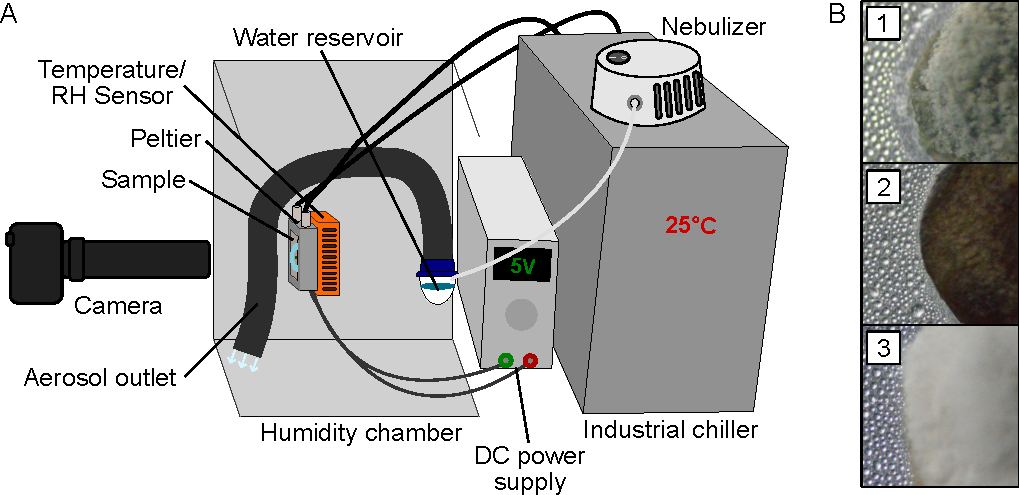
\includegraphics[width=\textwidth]{SuppFig1.pdf}
\caption{\textbf{Experimental setup and representative samples.} \textbf{(A)} Schematic of the sealed imaging chamber. A Peltier-cooled aluminum substrate ($T_s \approx 7\,^\circ$C) is thermally coupled to a closed-loop water chiller (CW-3000) via thermal paste. Silane-treated aluminum foil serves as the condensation surface. Water vapor is supplied by a compressor nebulizer (InnoSpire Essence, Respironics). Relative humidity and temperature are logged at 1-s resolution by a digital hygrometer--thermometer (IPT-100S, Elitech) with an external probe bound to the Peltier surface. Time-lapse imaging uses a DSLR camera on a motorized focus rail (StackShot, Cognisys) with LED illumination. \textbf{(B)} Representative brightfield images of samples on the cooled substrate: (1) a fungal colony patch, (2) a NaCl--agar hydrogel disk, and (3) an agar-only control. Circular patches are 3 mm in diameter.}
\label{fig:setup}
\end{figure}

\clearpage


\begin{figure}[H]
\centering
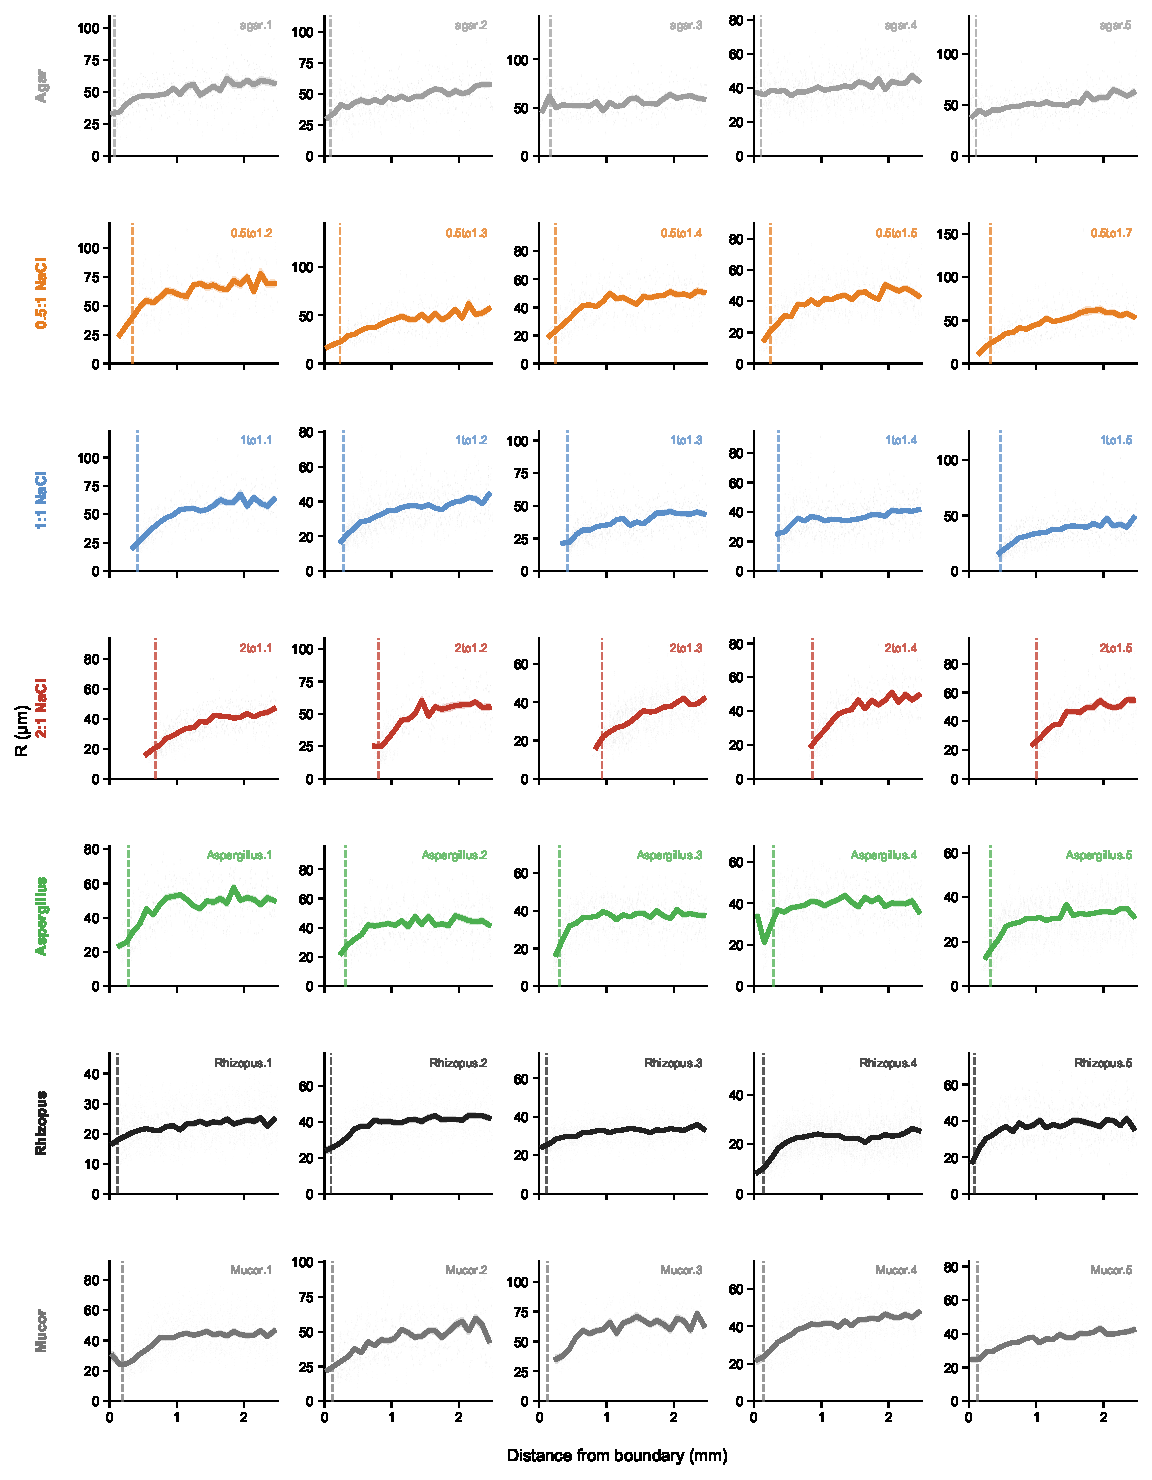
\includegraphics[width=0.85\textwidth]{SuppFig2.pdf}
\caption{\textbf{Normalized radial size profiles for all 35 laboratory trials.} Each panel shows one trial (7 conditions $\times$ 5 replicates). Gray scatter: individual droplet radii at $t = 14.5$--15.5 min versus distance from the source boundary. Colored band: mean $\pm$ SEM computed in 100 $\mu$m bins. Red dashed line: dry-zone width $\delta$. Trial identifier is shown in the top-right corner of each panel. Conditions (top to bottom): agar, 0.5:1 NaCl, 1:1 NaCl, 2:1 NaCl, \textit{Aspergillus}, \textit{Mucor}, \textit{Rhizopus}. The spatial size gradient---small near-field droplets transitioning to larger far-field droplets---is reproducible across all replicates and strengthens monotonically with increasing vapor-sink strength.}
\label{fig:Rd_all}
\end{figure}

\clearpage


\begin{figure}[H]
\centering
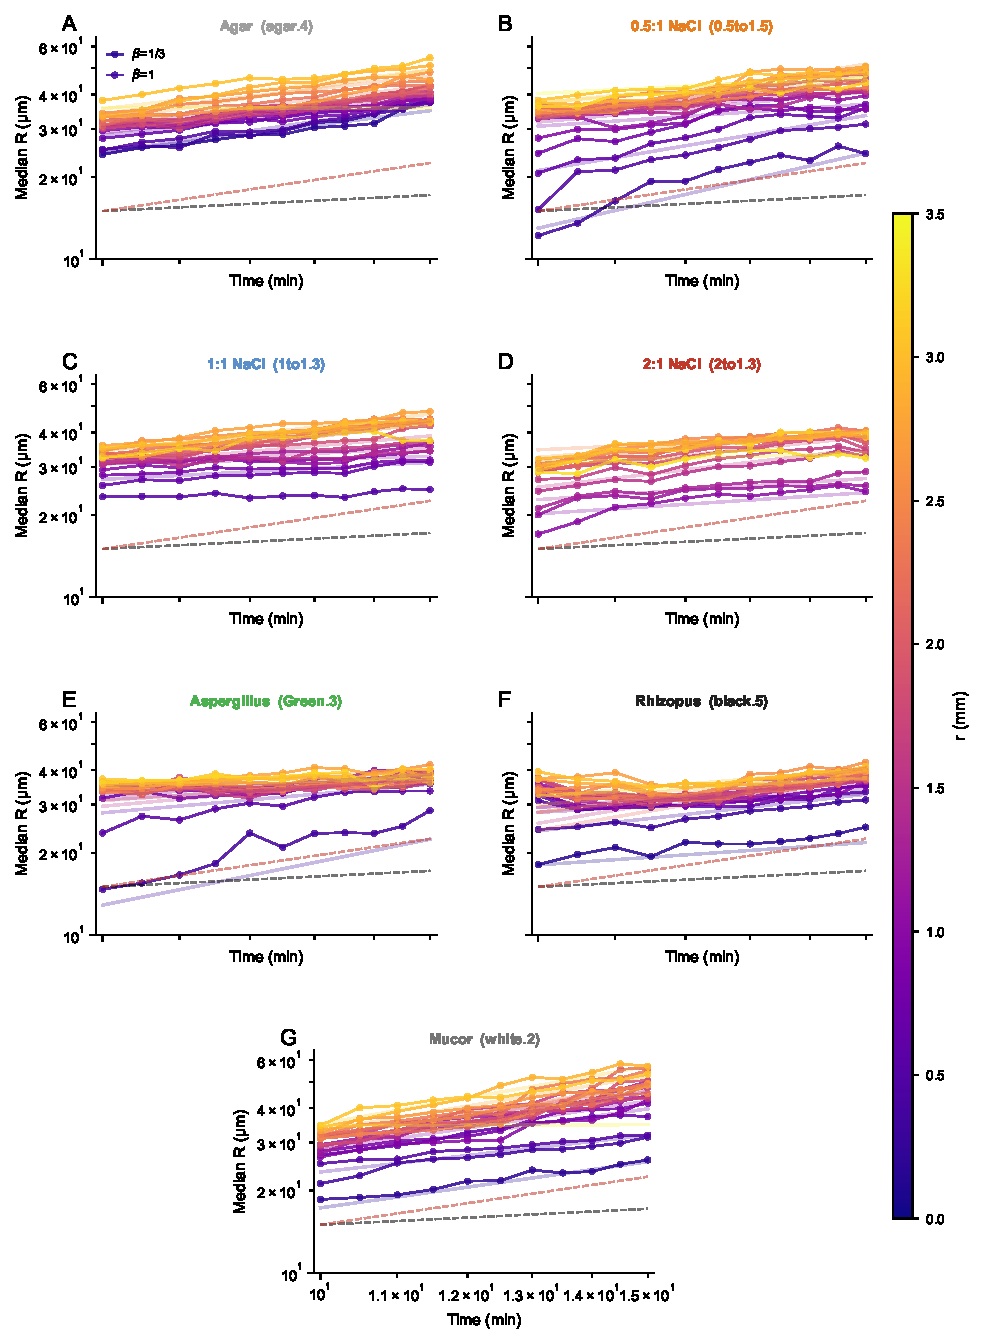
\includegraphics[width=0.8\textwidth]{SuppFig3.pdf}
\caption{\textbf{Droplet growth curves for all seven conditions.} Each panel shows one representative trial per condition (\textbf{A}--\textbf{G}). Log--log plot of median droplet radius $R$ versus time, with droplets binned by distance from the source boundary (plasma colormap; navy = near, yellow = far). Solid colored lines: fitted power-law slopes. Dashed reference lines: diffusion-limited scaling $R \propto t^{1/3}$ ($\beta = 1/3$, black) and coalescence-dominated scaling $R \propto t^{1}$ ($\beta = 1$, red). Near-field droplets track the $t^{1/3}$ regime for longer across all conditions, confirming that growth suppression in the depletion zone delays the transition to coalescence-dominated growth.}
\label{fig:beysens}
\end{figure}

\clearpage


\begin{figure}[H]
\centering
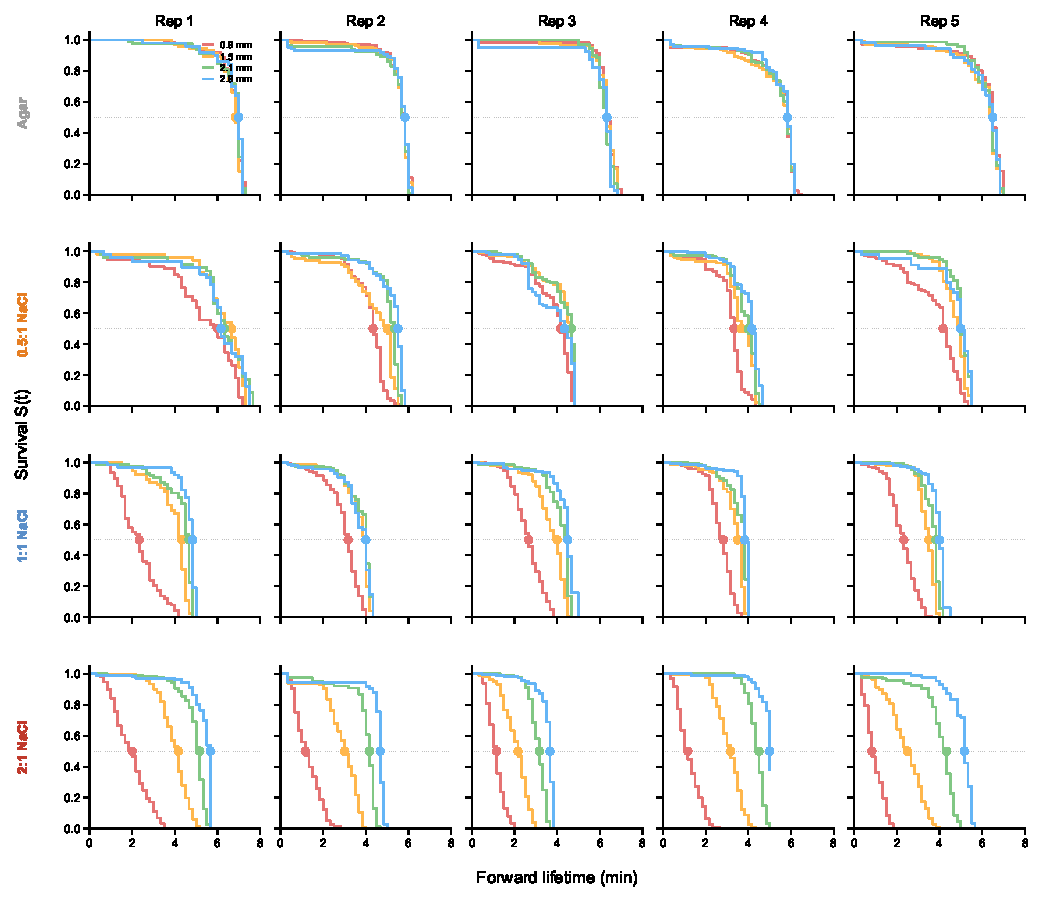
\includegraphics[width=\textwidth]{SuppFig4.pdf}
\caption{\textbf{Distance-stratified Kaplan--Meier survival curves for all 20 hydrogel trials.} Each panel shows one hydrogel trial (4 conditions $\times$ 5 replicates). Survival curves are stratified by four distance bands from the source boundary (0.9, 1.5, 2.1, and 2.9 mm). Dots mark the median survival time $\tau_{50}$ on the 0.5 survival line. Shaded bands: 95\% confidence intervals. Forward lifetimes are measured from evaporation onset ($t = 15$ min). Agar controls show flat or weakly separated curves; 2:1 NaCl trials show the strongest distance-dependent survival gradient. The monotonic decrease in $\tau_{50}$ with proximity to the source is present in every replicate of every NaCl condition, confirming the robustness of the temporal survival gradient.}
\label{fig:km_grid}
\end{figure}

\clearpage


\begin{figure}[H]
\centering
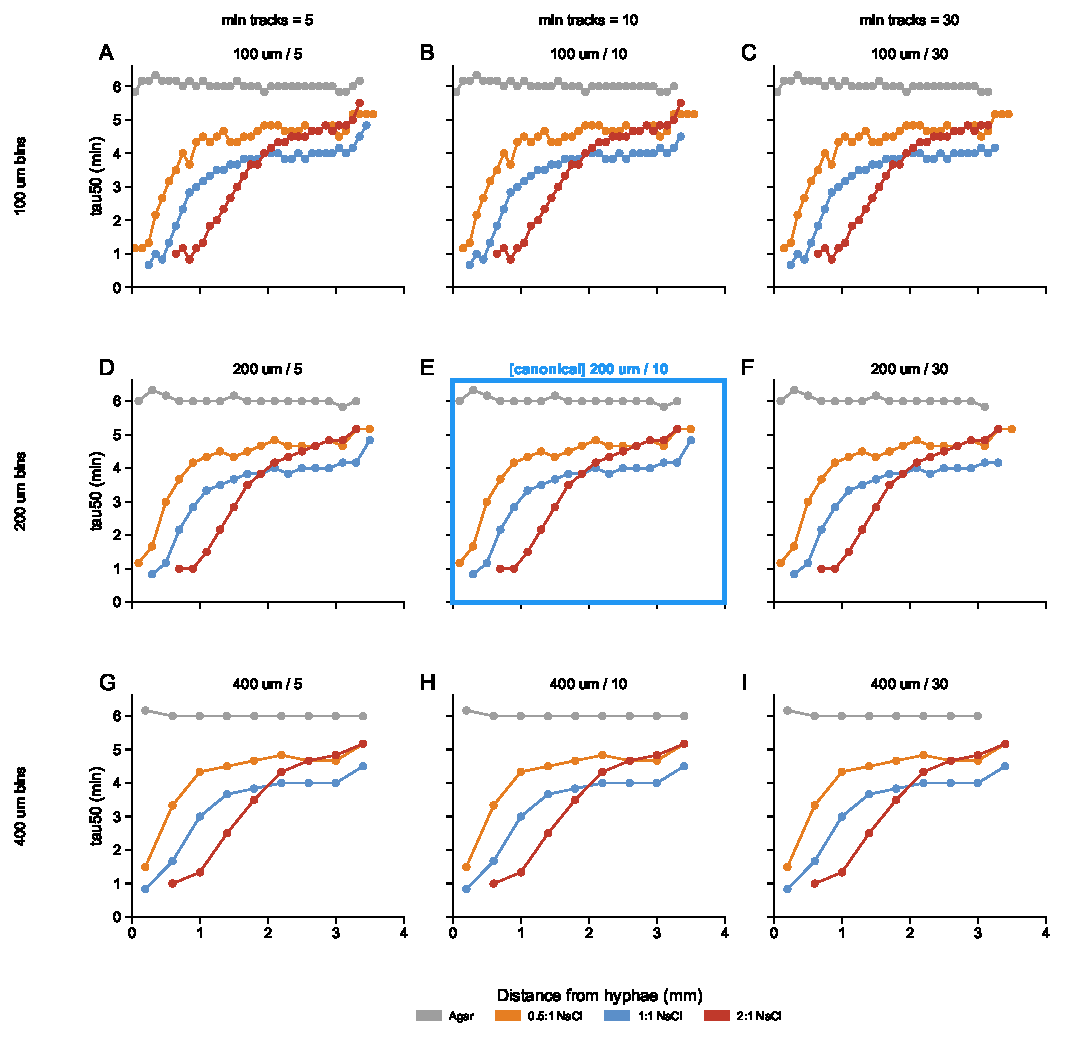
\includegraphics[width=\textwidth]{SuppFig5.pdf}
\caption{\textbf{Sensitivity of $\tau_{50}$--distance profiles to binning parameters.} $3 \times 3$ grid showing $\tau_{50}$ versus distance profiles for all four hydrogel conditions under nine combinations of bin width (100, 200, 400 $\mu$m) and minimum track count per bin (5, 10, 30). The canonical parameter set used in the main analysis (bin width = 200 $\mu$m, minimum tracks = 10; blue border) produces $\tau_{50}$ estimates that are consistent with alternative parameter choices. Profile shape and monotonic distance dependence are preserved across all nine combinations, confirming that the survival gradient metric is not sensitive to binning choices.}
\label{fig:km_sensitivity}
\end{figure}

\clearpage


\begin{figure}[H]
\centering
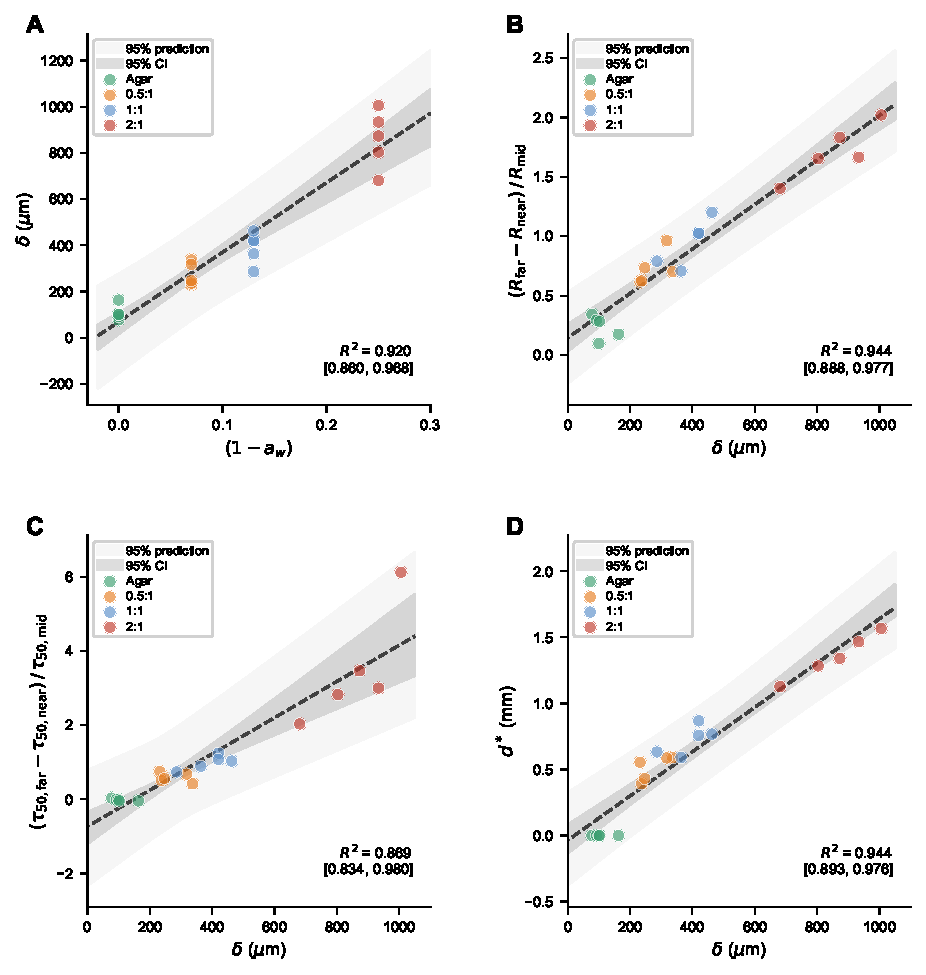
\includegraphics[width=\textwidth]{SuppFig6.pdf}
\caption{\textbf{Bootstrap confidence intervals for calibration regressions.} $2 \times 2$ panel grid showing the four calibration regressions from Fig.~2 with bootstrap 95\% confidence and prediction bands ($N = 10{,}000$ resamples). \textbf{(A)} Dry-zone width $\delta$ versus $(1 - a_w)$ (Fig.~2F). \textbf{(B)} Normalized size gradient $(R_{\mathrm{far}} - R_{\mathrm{near}})/R_{\mathrm{mid}}$ versus $\delta$ (Fig.~2H). \textbf{(C)} Normalized survival gradient $(\tau_{50,\mathrm{far}} - \tau_{50,\mathrm{near}})/\tau_{50,\mathrm{mid}}$ versus $\delta$ (Fig.~2K). \textbf{(D)} Half-attenuation distance $d^*$ versus $\delta$ (Fig.~2L). Dark shading: 95\% CI on the regression line; light shading: 95\% prediction interval. Points are colored by hydrogel group (agar, 0.5:1, 1:1, 2:1 NaCl). Inset $R^2$ values with bootstrap 95\% CIs confirm that all four linear relationships are statistically robust.}
\label{fig:bootstrap}
\end{figure}

\clearpage


\begin{figure}[H]
\centering
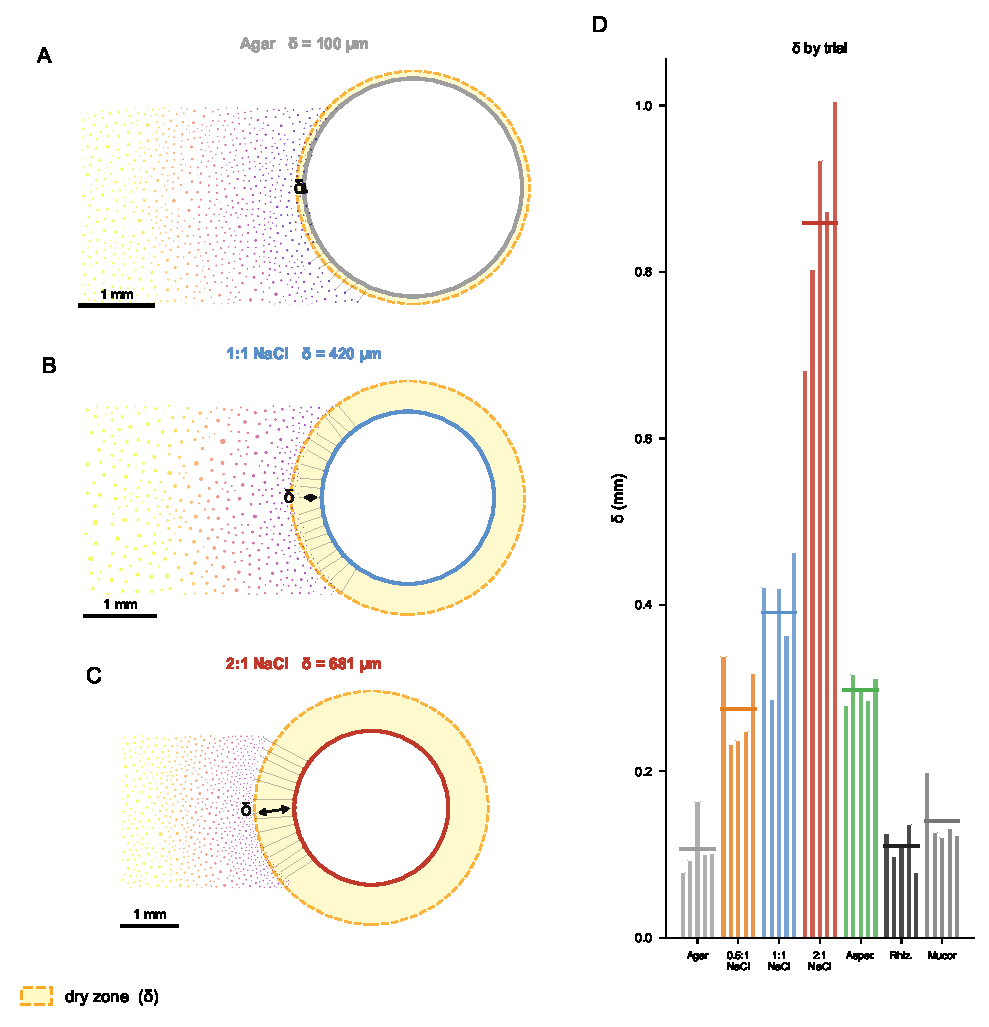
\includegraphics[width=\textwidth]{SuppFig7.pdf}
\caption{\textbf{Dry-zone width measurement by boundary raycast.} \textbf{(A--C)} Exemplar trials at three vapor-sink strengths: agar control ($\delta \approx 100$ $\mu$m), 1:1 NaCl ($\delta \approx 420$ $\mu$m), and 2:1 NaCl ($\delta \approx 681$ $\mu$m). Each panel shows the droplet scatter colored by distance from the source boundary, the traced boundary polygon, and raycast lines used to sample the minimum droplet-free distance along 100 equally spaced boundary points. \textbf{(D)} Bar chart of $\delta$ for all 35 laboratory trials, grouped by condition. $\delta$ increases monotonically with vapor-sink strength across both hydrogel and fungal conditions.}
\label{fig:raycast}
\end{figure}

\clearpage


\begin{figure}[H]
\centering
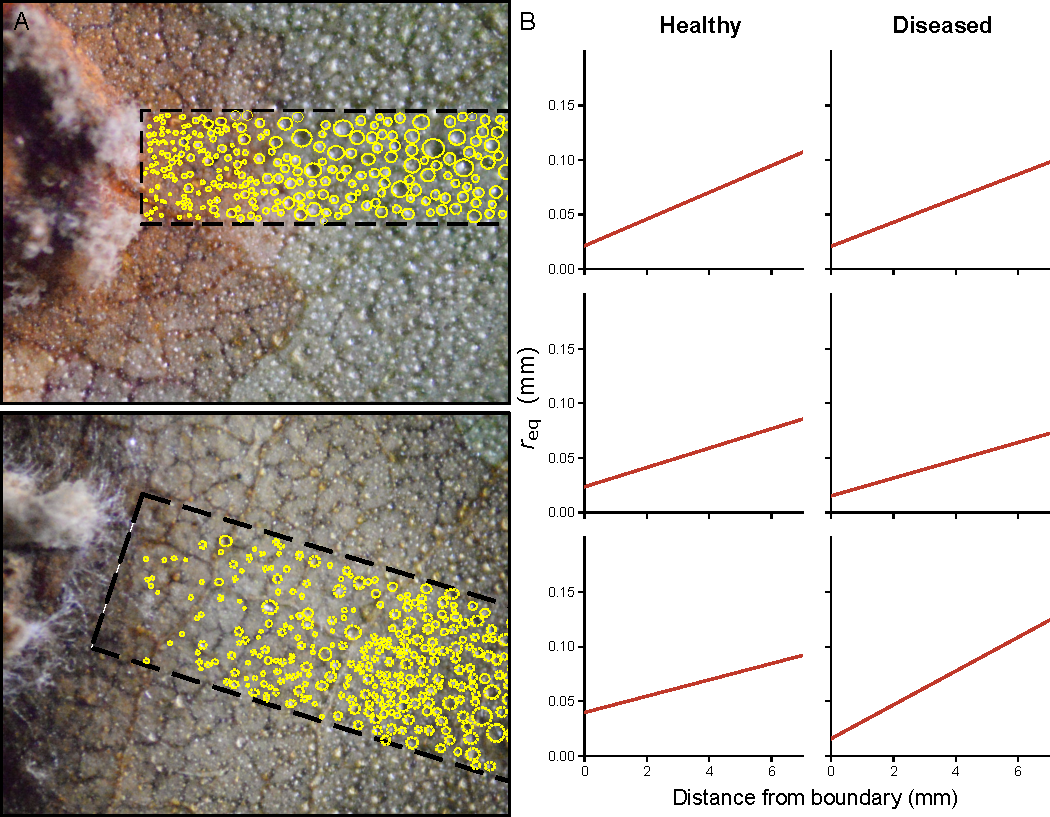
\includegraphics[width=\textwidth]{SuppFig8.pdf}
\caption{\textbf{Individual field trial size--distance scatter plots.} \textbf{(A)} Condensation micrographs of two \textit{Gymnosporangium yamadae}-infected \textit{Malus} leaf specimens with manual droplet annotations (red circles) and analysis regions (dashed rectangles). Top: healthy rust specimen. Bottom: diseased specimen with secondary fungal colonization. Scale bars: 3 mm. \textbf{(B)} Equivalent radius $r_{\mathrm{eq}}$ versus distance from the fungal boundary for each of the six field trials (3 healthy, left column; 3 diseased, right column). Gray dots: individual annotated droplets ($N = 1{,}507$ total). Red lines: ordinary least-squares regression. All six trials show a significant positive correlation between droplet size and distance (individual trial Pearson $r = 0.43$--0.66, all $p < 10^{-6}$; sign test for all-positive slopes: two-tailed $p = 0.031$).}
\label{fig:rsr_extended}
\end{figure}

\clearpage


\begin{table}[H]
\centering
\caption{\textbf{Sensitivity analysis of the normalized size gradient to zone boundary definitions.} The normalized size gradient $(\bar{R}_{\mathrm{far}} - \bar{R}_{\mathrm{near}})/\bar{R}_{\mathrm{mid}}$ was computed for 36 combinations of near, mid, and far evaluation zone boundaries and regressed against dry-zone width $\delta$ across all 35 laboratory trials (hydrogels + fungi). All combinations yield $R^2 \geq 0.87$ and Spearman $\rho \geq 0.79$, confirming that the metric is robust to the choice of zone boundaries. The canonical zone definitions used in the main text (near: 0--500 $\mu$m, mid: 900--1100 $\mu$m, far: 1900--2100 $\mu$m; bold) yield $R^2 = 0.916$.}
\label{tab:sensitivity}
\vspace{0.5em}
\small
\begin{tabular}{lllccc}
\toprule
Near ($\mu$m) & Mid ($\mu$m) & Far ($\mu$m) & $n$ & $R^2$ & $\rho$ \\
\midrule
0--700 & 900--1100 & 1700--2300 & 30 & 0.936 & 0.822 \\
0--700 & 900--1100 & 1500--2500 & 30 & 0.935 & 0.824 \\
0--700 & 900--1100 & 1900--2100 & 30 & 0.931 & 0.830 \\
0--1000 & 900--1100 & 1700--2300 & 30 & 0.926 & 0.815 \\
0--700 & 800--1200 & 1700--2300 & 30 & 0.925 & 0.822 \\
0--1000 & 900--1100 & 1500--2500 & 30 & 0.925 & 0.798 \\
0--700 & 750--1250 & 1700--2300 & 30 & 0.924 & 0.826 \\
0--700 & 800--1200 & 1500--2500 & 30 & 0.923 & 0.820 \\
0--700 & 750--1250 & 1500--2500 & 30 & 0.922 & 0.825 \\
0--500 & 900--1100 & 1700--2300 & 30 & 0.921 & 0.841 \\
0--500 & 750--1250 & 1700--2300 & 30 & 0.920 & 0.846 \\
0--1000 & 900--1100 & 1900--2100 & 30 & 0.920 & 0.817 \\
0--500 & 900--1100 & 1500--2500 & 30 & 0.920 & 0.841 \\
0--700 & 800--1200 & 1900--2100 & 30 & 0.920 & 0.821 \\
0--500 & 800--1200 & 1700--2300 & 30 & 0.919 & 0.843 \\
0--700 & 750--1250 & 1900--2100 & 30 & 0.918 & 0.833 \\
0--500 & 750--1250 & 1500--2500 & 30 & 0.917 & 0.841 \\
\textbf{0--500} & \textbf{900--1100} & \textbf{1900--2100} & \textbf{30} & \textbf{0.916} & \textbf{0.843} \\
0--500 & 800--1200 & 1500--2500 & 30 & 0.916 & 0.829 \\
0--500 & 750--1250 & 1900--2100 & 30 & 0.914 & 0.836 \\
0--500 & 800--1200 & 1900--2100 & 30 & 0.913 & 0.834 \\
0--1000 & 800--1200 & 1700--2300 & 30 & 0.903 & 0.812 \\
0--1000 & 800--1200 & 1500--2500 & 30 & 0.900 & 0.788 \\
0--1000 & 750--1250 & 1700--2300 & 30 & 0.899 & 0.812 \\
0--1000 & 800--1200 & 1900--2100 & 30 & 0.897 & 0.815 \\
0--1000 & 750--1250 & 1500--2500 & 30 & 0.896 & 0.790 \\
0--1000 & 750--1250 & 1900--2100 & 30 & 0.893 & 0.815 \\
0--300 & 750--1250 & 1700--2300 & 30 & 0.886 & 0.840 \\
0--300 & 750--1250 & 1500--2500 & 30 & 0.884 & 0.831 \\
0--300 & 750--1250 & 1900--2100 & 30 & 0.881 & 0.834 \\
0--300 & 800--1200 & 1700--2300 & 30 & 0.880 & 0.828 \\
0--300 & 800--1200 & 1500--2500 & 30 & 0.877 & 0.828 \\
0--300 & 800--1200 & 1900--2100 & 30 & 0.875 & 0.829 \\
0--300 & 900--1100 & 1700--2300 & 30 & 0.873 & 0.835 \\
0--300 & 900--1100 & 1500--2500 & 30 & 0.872 & 0.832 \\
0--300 & 900--1100 & 1900--2100 & 30 & 0.869 & 0.832 \\
\bottomrule
\end{tabular}
\end{table}

  \begin{figure}[H]                                                                                                                               
  \centering                                                                                                                                      
  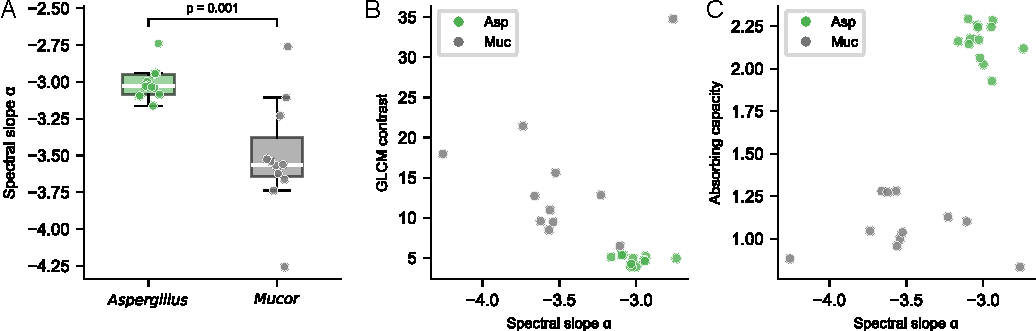
\includegraphics[width=\textwidth]{SuppFig9.pdf}
  \caption{\textbf{FFT spectral analysis cross-validates morphological metrics.} Tile-based 2D FFT ($256 \times 256$ px tiles, 128 px stride,     
  Hanning window) applied to all macro-scale brightfield colony-surface photographs (single-plane, not focus-stacked). \textbf{(A)} Mean radial   
  power spectra for \textit{Aspergillus} (green, $n = 13$) and \textit{Mucor} (gray, $n = 11$). Shaded region: frequency band used for slope      
  fitting (0.02--0.40 cycles/px). \textit{Aspergillus} retains more power at high spatial frequencies, indicating finer-grained surface texture.  
  \textbf{(B)} Spectral slope $\alpha$: \textit{Aspergillus} $= -3.01 \pm 0.11$, \textit{Mucor} $= -3.51 \pm 0.38$ (Welch's $t$-test, $p = 0.001$,
   $d = 1.85$; Mann--Whitney $U = 130$, $p = 0.0008$). Shallower slope indicates more sub-resolution surface roughness, consistent with the bumpy
  texture of packed conidial chains versus the smooth surfaces of \textit{Mucor} sporangiophores. \textbf{(C)} Cross-validation: $\alpha$ versus
  GLCM contrast across all ROIs (Spearman $r = -0.63$, $p = 0.0009$). Two independent texture methods (frequency-domain and spatial-domain)
  converge on the same genus ordering. Spearman is reported because the relationship is monotonic but the Pearson estimate is sensitive to a
  single high-contrast \textit{Mucor} ROI. \textbf{(D)} $\alpha$ versus absorbing capacity (Spearman $r = 0.49$, $p = 0.014$). Colonies with
  shallower spectral slope (more textured surfaces) also present higher absorbing capacity, linking sub-resolution roughness to effective
  vapor-sink strength.}
  \label{fig:supp_fft}
  \end{figure}

  \clearpage                                                                                                                                      
   
                                                                                                                                                  
  \begin{figure}[H]                                                   
  \centering
  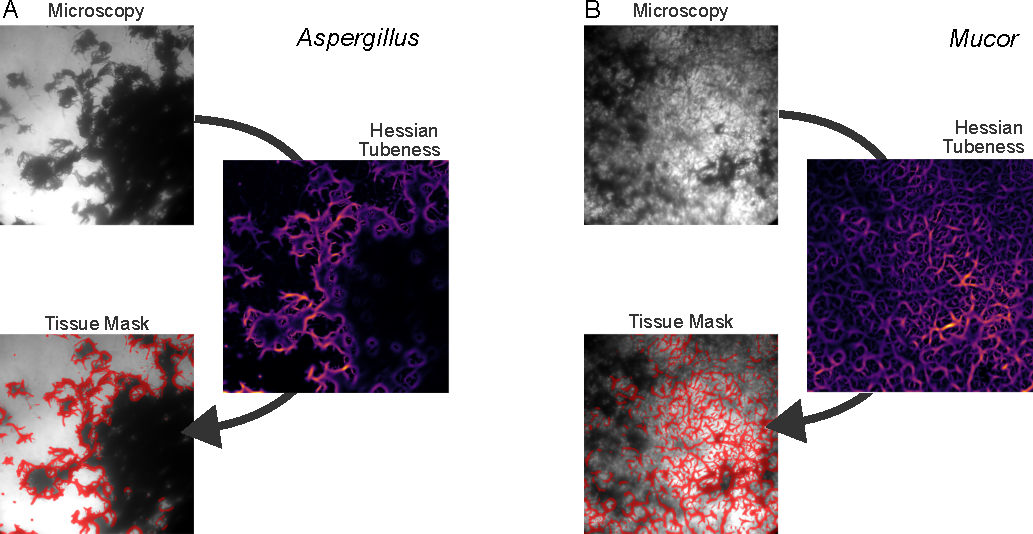
\includegraphics[width=\textwidth]{SuppFig10.pdf}
  \caption{\textbf{Multi-scale Hessian tubeness on light microscopy.} Representative $10\times$ fields: \textit{Aspergillus} (Pink\_10X\_1.TIF,
  \textbf{A}) and \textit{Mucor} (White\_10X\_1.TIF, \textbf{B}). Each 4-panel overlay shows: original transmitted-light image (top-left);        
  multi-scale Hessian tubeness response ($\sigma = 1, 2, 4, 8, 16$ px, maximum across scales; inferno colormap, top-right); detected tubular
  structures (red overlay, bottom-left); internal classification (blue = solid tissue, yellow = internal pores, bottom-right). Hessian tubeness   
  selectively responds to elongated filamentous structures. \textit{Mucor}'s sparse hyphal network produces a uniform, high tubeness response
  (foreground fraction = 0.276), while \textit{Aspergillus}'s dense conidial masses register low tubeness except at filamentous edges (foreground
  fraction = 0.185), consistent with packed rather than filamentous architecture. The Hessian tubeness ``foreground fraction'' reported here is
  intentionally selective for filamentous structures and rejects \textit{Aspergillus}'s dense conidial cores; this differs from the
  adaptive-threshold tissue fraction $f_\mathrm{tissue}$ reported in Supplementary Fig.~\ref{fig:supp_capacity}A ($f_\mathrm{tissue,Asp} = 0.300 >
   f_\mathrm{tissue,Muc} = 0.258$), which captures all dark tissue including cores. \textit{Aspergillus}'s lower Hessian-foreground but higher
  adaptive-tissue fraction is internally consistent and is the underlying reason its tubeness CV is high (Supplementary
  Fig.~\ref{fig:supp_tubcv}).}
  \label{fig:supp_hessian}
  \end{figure}

  \clearpage


  \begin{figure}[H]
  \centering
  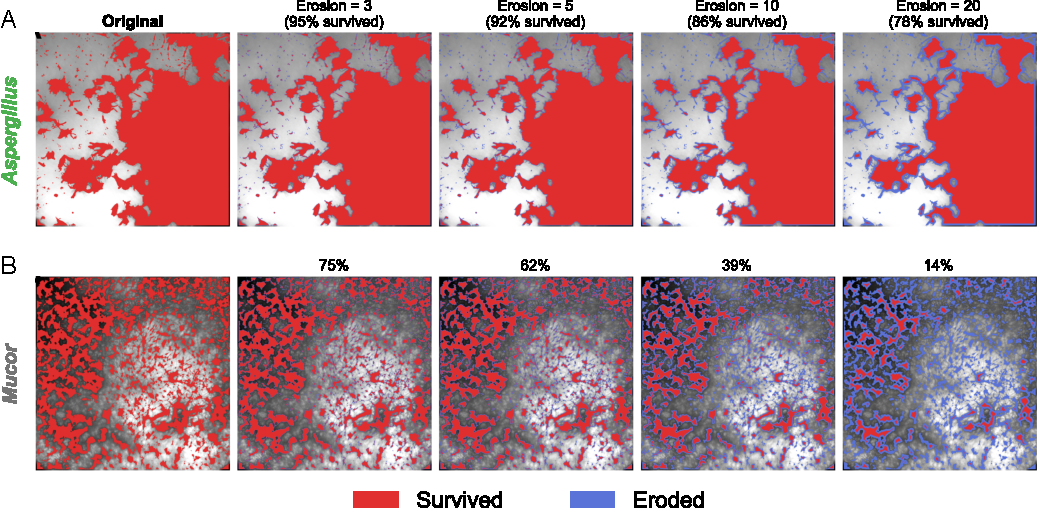
\includegraphics[width=\textwidth]{SuppFig11.pdf}                                                                                               
  \caption{\textbf{Progressive morphological erosion.} Adaptive-segmented tissue masks subjected to 0, 2, 5, 10, and 20 iterations of binary
  erosion. Red = tissue surviving erosion; blue = tissue eroded away. \textbf{(A)} \textit{Aspergillus} (Pink $10\times$). Dense conidiospore     
  cores persist through 20 iterations (survival at 10 iterations $= 86\%$). \textbf{(B)} \textit{Mucor} (White $10\times$). Thin hyphal filaments
  are substantially eroded by 10 iterations (survival at 10 iterations $= 39\%$). Erosion survival quantifies structural persistence: thick,      
  packed tissue withstands more erosion cycles than thin filaments. Overall: \textit{Aspergillus} $= 0.791 \pm 0.103$, \textit{Mucor} $= 0.372 \pm
   0.025$ (Welch's $t$-test, $p = 7.9 \times 10^{-5}$, $d = 4.75$; Mann--Whitney $U = 18$, $p = 0.024$ --- bounded by $n_a = 6$, $n_m = 3$).
  Erosion survival values reported in the main text are the per-ROI tissue-retention fraction at erosion iteration 10, averaged across ROIs ($n =
  6$ \textit{Aspergillus}, $n = 3$ \textit{Mucor}).}
  \label{fig:supp_erosion}
  \end{figure}

  \clearpage


  \begin{figure}[H]
  \centering
  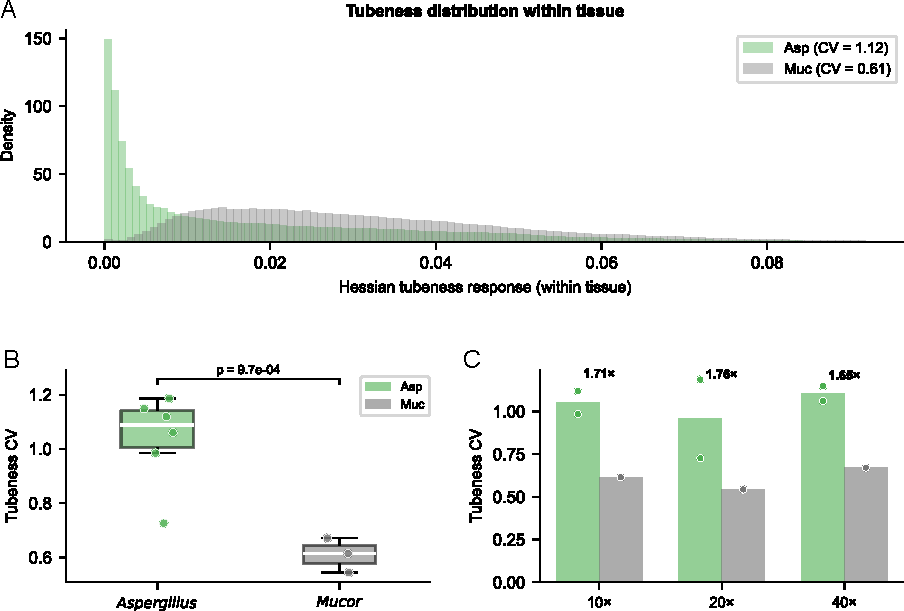
\includegraphics[width=\textwidth]{SuppFig12.pdf}
  \caption{\textbf{Hessian tubeness CV derivation.} \textbf{(A)} Distribution of multi-scale Hessian tubeness response within tissue pixels for   
  one representative ROI per genus (\textit{Aspergillus}, green, single-ROI CV $= 1.12$; \textit{Mucor}, gray, single-ROI CV $= 0.61$); the       
  all-image means are reported in panel B. Dashed lines mark means. \textit{Aspergillus} tissue has a broader, more heterogeneous                 
  distribution---reflecting a mix of solid conidial cores (low tubeness) and filamentous edges (high tubeness)---while \textit{Mucor} tissue is   
  narrowly distributed around a single filamentous mode. The \textit{Aspergillus} distribution is strongly bimodal (a zero-inflated peak from
  solid conidial cores plus a high-tubeness tail from filamentous edges), so the high CV reflects this two-mode structure rather than a wider
  unimodal distribution. \textbf{(B)} Tubeness CV across all light-microscopy images: \textit{Aspergillus} $= 1.04 \pm 0.17$, \textit{Mucor} $=
  0.61 \pm 0.06$ (Welch's $t$-test, $p = 9.7 \times 10^{-4}$, $d = 2.93$; $n = 6$ vs.\ $n = 3$). Mann--Whitney $U$ is bounded by $p \geq 0.024$ at
   $n_a = 6$, $n_m = 3$ (limited by sample size); Welch's $t$ is reported as primary because the per-image tubeness CV is approximately Gaussian
  within group. The CV is computed within a class-specific adaptive-threshold tissue mask; replacing the class-specific operator with a single
  universal segmentation reduces the Asp/Muc ratio to $1.20$ ($p = 0.17$). \textbf{(C)} Magnification independence: the Asp/Muc ratio is preserved
   at $1.71\times$ ($10\times$), $1.76\times$ ($20\times$), and $1.65\times$ ($40\times$).}
  \label{fig:supp_tubcv}
  \end{figure}

  \clearpage


  \begin{figure}[H]
  \centering
  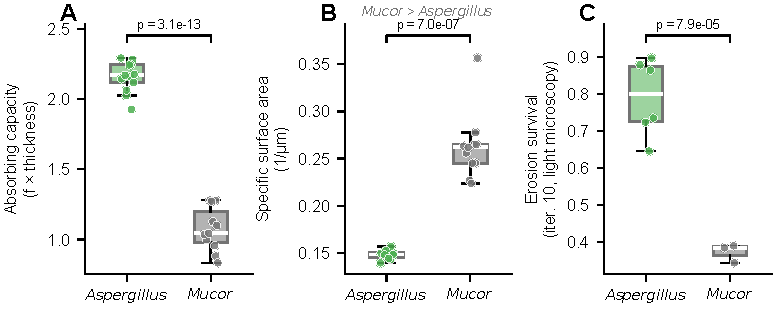
\includegraphics[width=\textwidth]{SuppFig13.pdf}
  \caption{\textbf{Absorbing capacity decomposition and specific surface area.} Per-ROI strip charts for the components of absorbing capacity $\mathcal{A} = f_\mathrm{tissue} \times d_\mathrm{structure}$. \textbf{(A)} Tissue fraction $f_\mathrm{tissue}$: \textit{Aspergillus} $= 0.300 \pm 0.008$, \textit{Mucor} $= 0.258 \pm 0.019$ (ratio $= 1.16$, $p = 1.1 \times 10^{-5}$). \textbf{(B)} Structure thickness                     
  $d_\mathrm{structure}$ (median distance transform, $\mu$m): \textit{Aspergillus} $= 7.21 \pm 0.26$, \textit{Mucor} $= 4.16 \pm 0.53$ (ratio $=  
  1.73$, $p = 7.1 \times 10^{-11}$). \textbf{(C)} Absorbing capacity $\mathcal{A}$: \textit{Aspergillus} $= 2.16 \pm 0.11$, \textit{Mucor} $= 1.07
   \pm 0.16$ (ratio $= 2.01$, $d = 8.22$, $p = 3.1 \times 10^{-13}$). Their product predicts the measured $\delta$ ratio (2.13) within $6\%$.     
  \textbf{(D)} Specific surface area (tissue--air boundary per tissue area): \textit{Mucor} $= 0.262 \pm 0.035$ $\mu$m$^{-1}$,               
  \textit{Aspergillus} $= 0.148 \pm 0.005$ $\mu$m$^{-1}$ ($p < 10^{-6}$). Despite $1.78\times$ higher surface-to-volume ratio, \textit{Mucor} is
  the weaker sink: total hygroscopic mass per colony footprint, not surface-to-volume ratio, determines effective sink strength. $n = 13$       
  \textit{Aspergillus}, $n = 11$ \textit{Mucor} ROIs.}                                                                                   
  \label{fig:supp_capacity}                           
  \end{figure}             
                                                                                                                                                  
  \clearpage
                                                                                                                                                  
                                                                      
  \begin{figure}[H]
  \centering       
  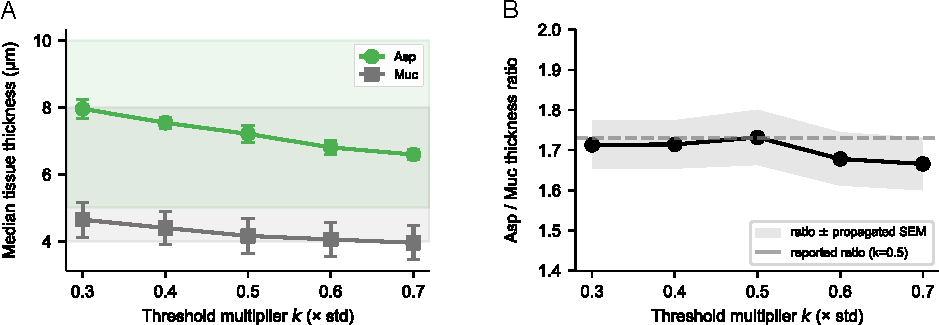
\includegraphics[width=\textwidth]{SuppFig14.pdf}
  \caption{\textbf{Segmentation threshold sensitivity for macro-scale colony-surface masks.} Adaptive dark-response thresholding (smooth $\sigma =
   1$ px, local mean $\sigma = 32$ px) was swept over threshold multipliers $k = 0.3$ to $0.7\,\times$ std on the same 13 \textit{Aspergillus} and
   11 \textit{Mucor} ROIs used in the main analysis. \textbf{(A)} Median tissue thickness as a function of $k$ for both genera (mean $\pm$ std    
  across ROIs). Shaded bands: published hyphal-diameter ranges (\textit{Aspergillus} conidiophore stipe and conidial-chain width 5--10 $\mu$m,    
  green; \textit{Mucor} sporangiophore-segment width 4--8 $\mu$m, gray). Both genera fall within their published ranges across the entire sweep,  
  supporting the calibration choice. \textbf{(B)} Asp/Muc thickness ratio is stable at $1.67$--$1.73$ across the full sweep ($k = 0.3$--$0.7$),
  with the propagated SEM band (relative quadrature on independent group means) overlapping the reported ratio across all thresholds. The Welch
  $p$-value remains $< 2.4 \times 10^{-9}$ at every threshold tested. Tabulated values are in \texttt{segmentation\_sensitivity.csv} (OSF
  deposit).}
  \label{fig:supp_seg3d}
  \end{figure}

  \clearpage

\end{document}
